% Standalone figure for the Statistical Mechanics notes.
% Build: pdflatex binary-PX.tex  (or run build.sh in this folder)
\documentclass[11pt,tikz,border=2pt]{standalone}
\usepackage{amsmath,amssymb}
\usetikzlibrary{arrows.meta, positioning}
\begin{document}
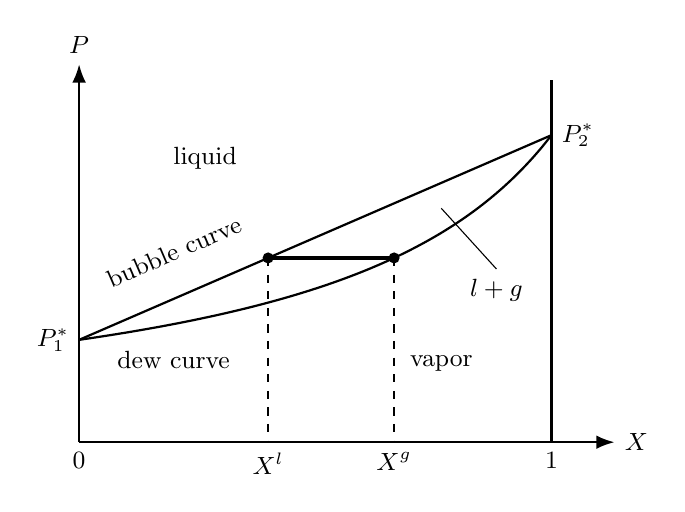
\begin{tikzpicture}[font=\small, >=Latex, line width=0.8pt]
    % axes: x = 6X, y = 1.3P; P_1^* = 1, P_2^* = 3
    \draw[->] (0,0) -- (6.8,0) node[right] {$X$};
    \draw[->] (0,0) -- (0,4.8) node[above] {$P$};
    \draw (6,0) -- (6,4.6);
    \node[below] at (0,0) {$0$};
    \node[below] at (6,0) {$1$};
    % bubble curve (linear) and dew curve
    \draw (0,1.3) -- (6,3.9);
    \draw[domain=0:1, smooth, samples=50, variable=\t]
        plot ({6*\t},{1.3/((1-\t)+\t/3)});
    \node[left] at (0,1.3) {$P_1^*$};
    \node[right] at (6,3.9) {$P_2^*$};
    % tie line at P = 1.8 for overall X = 0.5
    \draw[line width=1.6pt] (2.4,2.34) -- (4.0,2.34);
    \fill (2.4,2.34) circle (2pt);
    \fill (4.0,2.34) circle (2pt);
    \draw[dashed] (2.4,2.34) -- (2.4,0) node[below] {$X^l$};
    \draw[dashed] (4.0,2.34) -- (4.0,0) node[below] {$X^g$};
    % labels
    \node at (1.6,3.6) {liquid};
    \node at (4.6,1.0) {vapor};
    \draw[line width=0.4pt] (4.6,2.97) -- (5.3,2.2) node[below] {$l+g$};
    \node[rotate=23.4, above] at (1.3,2.2) {bubble curve};
    \node at (1.2,1.05) {dew curve};
\end{tikzpicture}
\end{document}
